\section{Code Generation}
\label{sec:implementation_codeGen}
To generate the target code, first, the parse tree is traversed and the source code is translated to an in-memory representation consisting of objects corresponding to different language concepts. These concepts can be divided into three different kinds: statements, declarations, and code blocks. All of the objects implement the \texttt{ITranslatable} interface; it requires a translation function that translates the source code representation to the target code representation. In turn, they are often referred to as translatables. The target code representation is a collection of objects that describe an OpenQASM program; they can be translated directly to the textual OpenQASM code. In the following, we discuss the generation of the source code representation from the parse tree, the translation from the source code to the target code representation, and any other utilities that are used in the process.

\subsection{Source Code Representation}
\label{sec:implementation_sourceCode}
Similar to the implementation of the semantic analysis, the parse tree is traversed with another custom listener. However, in contrast to the semantic analysis, the code generation listener does not directly interact with a symbol table but uses a separate code generation handler.

The code generation handler facilitates the creation of the source code representations when traversing the parse tree. Firstly, it contains a main code block; this code block is initiated as an empty code block without a parent when the handler is created. Furthermore, it will hold, directly or indirectly, the references to all other source code objects. The second important property is the symbol table. The handler implements different methods for interacting with this table. For example, it contains methods for both pushing and popping scopes as well as guards. Additionally, the handler implements unique functions for each symbol that can be added to the table, with a protected general function. This is done because some symbols need additional logic when they are added to the symbol table. For example, when a register symbol is added to the table, a register declaration is also added to the current code block.

In the code generation listener, similar to the semantic analysis, the scopes and guards are pushed and popped based on the tree traversal. Furthermore, the symbols are also added according to the declarations in the source code. Except for the main code block, all translatables, \ie, code blocks, statements, and declarations, belong to exactly one code block. In turn, whenever one is reached in the traversal of the parse tree, the translatable is created and added to the corresponding code block. This code block is always identified as the current code block. Whenever a code block is entered, the current code block is updated to the newly created one. In turn, when a block is exited, the current is set to the parent block of the current one.

The first example of a translatable is the register declaration; as described previously, whenever a register symbol is added, the corresponding declaration is added to the current code block. In contrast, statements require more information. For each statement, the relevant symbol information is read from the symbol table based on the given identifier. Furthermore, any additional information is retrieved from the code generation handler. Then, both the symbol and additional information are used to create the statement object. For example, a loop statement requires both the loop iterator symbol and the code block object of its loop body. In turn, since the code block needs to have been traversed, the loop statement is created in the exit function of the loop rule. However, as the code block already existed, the listener class needs to save the last popped scope and retrieve the code block, corresponding to the loop body, from it. The loop iterator can easily be read from the symbol table based on the given identifier. While the type checking ensures the correct type of the symbol in most cases, a code generation exception may be thrown if the symbol in the table is not a loop iterator. Finally, the loop statement is created and added to the code generation handler and, in turn, to the current code block. The creation of the other statements works similarly; however, since the predefined and composite gates are implemented as separate translatable statements, the gate applications need to differentiate between the two and create the corresponding statement.

The most basic translatable is the code block. It represents a block of code in the source program and, in turn, contains all statements and declarations contained in the block; they are saved in a list of translatables. Next, the code block object also contains a reference to its parent code block. If the code block is the main block of the program, the parent is set to null. While each variable has a unique identifier, this identifier is only unique in the context of its declaration, and an independent context may contain a declaration for the same identifier. Therefore, the identifiers used in the source code may not be usable in the target code. To solve this issue, each declaration is assigned a new unique identifier. The code block contains a dictionary that maps all its declarations to the corresponding unique identifiers. Besides these three properties, the code block implements some functions to add translatables to the list and some utility functions to, \eg, retrieve the unique identifiers for declarations.

Another type of translatable is the declaration. While there are multiple different declarations, \eg, register and composite gate declarations, in our source language, most concepts are not translated to a corresponding declaration in the target language; in turn, there currently exists only one possible declaration. However, for extensibility, the compiler contains an abstract declaration class; it includes a symbol property with a reference to the symbol that is declared by the object. The register declaration inherits from the abstract class.
The third group of translatables is statements. Each statement inherits from an abstract statement class. Each statement contains an error context that corresponds to the source code location of the statement. In total, there are six different statements. 

The first two are the different gate application statements, the composite gate statement and the gate application statement. Since the implementation of the translation differs so greatly, they are implemented as two different statements. Both contain a gate property; however, while the gate property of the composite gate statement is a composite gate, the gate application contains a predefined gate in its property. Furthermore, they both contain an arguments property. In this case, while the gate application statement simply saves a list of symbols, the composite gate contains a dictionary that maps the argument symbols used in the composite gate to the symbols given as arguments.

Next, three statements are related to the control flow of the program. Firstly, the loop statement contains both the loop iterator symbol and the body of the loop in the form of a code block. Similarly, the quantum if-statement also contains a reference to its code block. Additionally, the statement includes a guard property that holds the symbol guarding the execution of the code block. Lastly, the else-statement simply inherits from the if-statement and contains no additional properties, only differing in the translation implementation.

Lastly, in contrast to most other statements, the skip statement does not contain any additional properties. All the different translatables, including the code block, statements, and declarations, are depicted in Fig.~\ref{fig:implementation_uml_translatables}. 

\begin{figure}[htp]
    \centering
    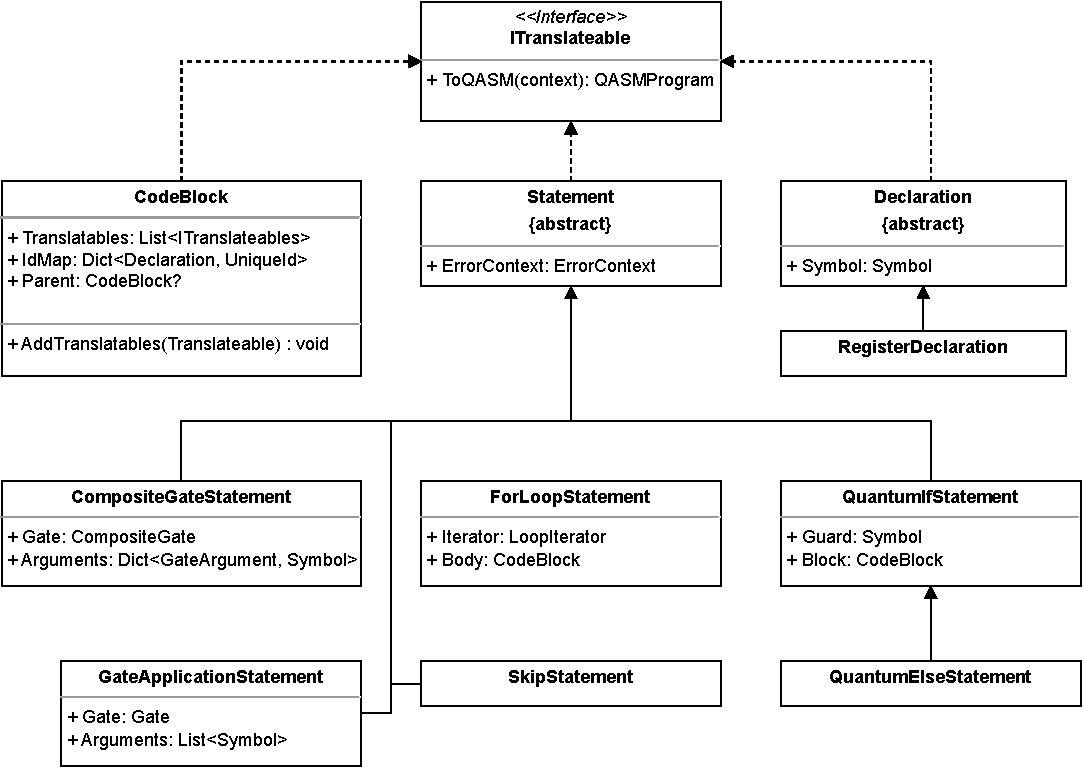
\includegraphics[width=.9\textwidth]{../figures/drawio/uml_translateables.pdf}
    \caption{A diagram showing the hierarchy of translatable classes.}
    \label{fig:implementation_uml_translatables}
\end{figure}

\subsection{Translation}
\label{sec:implementation_translation}
To create the target code representation that can be translated to the final program, the translatables, \ie, code blocks, declarations, and statements, need to be translated. For this, all translatables implement a translation function that takes the code generation context and returns the target code representation in the form of a \texttt{QASMProgram} object.

The code generation context contains all additional, relevant information for the code generation that is not already contained in the translatable objects themselves; this may include information that is not known at the time the translatables are created and instead injected when they are translated. The first property is the current block, which holds a reference to the code block for which the code is generated. Since all statements must be contained in a block, there must also always exist a current code block. The block, \eg, contains a dictionary that maps declarations to their new unique identifiers; this dictionary is filled while translating the declarations. Therefore, this information must be injected at generation time with the help of the code generation context. 

Similarly, the code generation context holds the symbol table that is generated while creating the source code representation. However, this symbol table may be changed while the code is translated. For example, composite gates are inlined where they are applied. However, the translation of the composite gate requires an empty symbol table, as they do not have access to any symbols outside the scope of the composite gate. In turn, the translation of the composite gate cannot use the symbol table of its current block but must create a new one. The symbol table itself is used to retrieve symbol information for, \eg, the evaluation of expressions where it may be used to get the value of a constant symbol.

Lastly, the context contains a dictionary that maps an argument to a symbol. This is used for the translation of the composite gates. Since there may exist nested composite gates, \ie, a composite gate that calls another composite gate, the dictionary contained in each composite gate statement is not sufficient for the translation alone. In turn, for each composite gate translation, the corresponding mappings are added to the dictionary.

The translation of any source code representation will always start with a code block translation, as it is always the root of a program. However, our target code representation does not contain a code block equivalent. In turn, instead of translating the code block directly, a new program object is created, and each translatable, contained in the code block, is translated individually and appended to the program object. Then, the result is returned.

In contrast, the register declaration has an equivalent in the target language. In this case, this is the qubit declaration code. However, as previously described, the identifier that is declared may not be unique. In turn, the symbol table is used to create an identifier that is unique in the resulting program. For this, a static integer is used and incremented. Furthermore, this identifier is added to the dictionary of the current block so that any reference to the declaration can be mapped to the newly created unique identifier. While the size of a register declaration is given in the form of an expression, the target code object requires a constant integer value. Therefore, the size expression is also evaluated before the code object is created. 

Of the statements, the skip statement is the easiest to translate; it represents an empty operation and, therefore, is translated by returning an empty program object. Similarly, the gate application statement has a simple translation. Since the target language also contains gate application statements, the translation simply needs to convert the gate and arguments to the target code representation. This can be accomplished with some simple helper functions and lookups. In contrast, the composite gate statement does not have any target code equivalent and is, instead, inlined. In turn, the composite gate translation simply calls the translation for the body code block and injects some argument mappings. Then, the translation of the body is returned.

The translation of the loop statements is, in principle, similar to the translation of a composite gate; it also contains a code block that is translated. However, the code block is not inlined once but needs to be translated multiple times, each time with a different value for the iterator. To achieve this, both the start index and end index expressions are evaluated. Next, the current value of the iterator is set to the start index, and a for loop is executed until the current value is equal to or larger than the end value. For each iteration, the code block is translated and added to a program. At the end, the program consists of the unrolled loop statement and is returned. 

Lastly, the translations of the if- and else-statements are mostly identical. In our target language, OpenQASM, the desired behavior for both the if- and else-statements can be accomplished by adding a control and negative control to each gate application statement in the code block, respectively. For this, the program object contains a function to add a guard. In this function, all code objects are iterated, and the guard is added to each gate application code. For the else-statement, a negated guard is added. Therefore, the translation of the if- and else-statements consists of translating the code block and adding the guard symbol as a possibly negated guard to it. 

\subsection{Target Code Representation}
\label{sec:implementation_targetCode}
The target code is translated from the source code representation in the form of a \texttt{QASMProgram} object. This program object functions as a wrapper for the translated gate applications and declarations and, in turn, holds a list of \texttt{Code} objects that represent these translations. Additionally, it provides functions to add and optimize the program or print the final target code string. 

Each code object inherits from the abstract code class, which implements two abstract functions. The first is a \texttt{ToCode} function, which converts the object to code by returning the text string of the code object. Secondly, the class implements a function that checks the semantic equivalence of a given code to the code object. In this case, if two code objects result in the same behavior of the program, they are semantically equal. For example, two gate applications are equal if they apply two semantically equivalent gates and the arguments and guards are semantically equivalent. The semantic equivalence is used in the optimization rules to check whether different rules are applicable. In the following, we will discuss the different code classes and their implementation. 

The main two code classes are the gate application code and qubit declaration code. The gate application code represents a gate application and, in turn, contains the guards for the gate, an object that represents the gate, and a list of qubit arguments to the gate. All these different properties have their own code classes, guard codes, gate codes, and qubit codes, respectively. For the code conversion, the gate application adds the control and negative control depending on the number of positive, \ie, not-negated, guards and negative guards, respectively. Next, the gate is converted and added. If they exist, both the positive and negative guards are converted, joined by commas, and added to the code. Similarly, at the end, the arguments are translated and added, separated by commas, to the code string. To check the equivalence of two gate applications, first, the arguments are checked. 
Since the order of arguments matters, both argument lists are iterated simultaneously, and the equivalence of each argument pair is checked. In contrast, the order of guards does not matter; in turn, it suffices that, for each guard in one list, there exists a guard in the other that is semantically equal. Lastly, the equivalence of the gates is checked. 
Additionally, when a gate code is created, some extra checks and transformations are performed. Firstly, a check is performed that qubits used as guards are disjunct from the qubits used as arguments to the gate. As for the transformations, any use of a controlled-not or Toffoli gate is replaced with an $X$ gate, and the control qubits are added to the guards; while the circuit description remains equivalent, any transformations in the following optimization stage do not require additional cases to find different kinds of controlled-not gates.

The guard code holds a reference to the qubit code that guards the gate as well as a boolean value that indicates whether the guard is negated or not. Two guard codes are semantically equivalent if their corresponding qubits are and their negation status matches. The code conversion just references the conversion of the qubit.
Next, the gate code holds the gate type, the code conversion prints the gate based on the type, and the semantic equivalence compares the gate type. Additionally, there exists a parameterized gate that inherits from the gate code class. In this case, the object holds an additional parameter property, and functions are adjusted accordingly. Lastly, the qubit code class holds a reference to the register symbol it is associated with for error handling and the unique identifier of the qubit in the target code. The code conversion simply returns the unique identifier, and the semantic equivalence compares the identifiers. Additionally, there exists a register access code that inherits from the qubit code. It contains an extra index property. In the semantic equivalence function, the base function is called, \ie, the equivalence function of the qubit code, and the indices are compared. Furthermore, the code conversion returns an access to the identifier based on the index property.

The declaration code is an abstract class that represents any declaration in the OpenQASM program. It contains a unique identifier property for the variable it declares. Additionally, with the identifier, the class can also implement the semantic equivalence check where the identifiers are compared. The qubit declaration code inherits from the class and contains an additional size property, corresponding to the size of the register. Depending on the size of the declaration, either a single qubit is declared in the conversion, if the size is one, or a quantum register for the given size is declared.

While the gate application and qubit declaration code, as well as the related classes, are sufficient to translate the source code, the resulting program does not contain any measurements. Since our language only supports implicit measurements, these are added after the translation and optimization of the code. More specifically, the program class contains a function that prints the final program with the required OpenQASM header and adds measurements for each qubit and register in the circuit; when the compiler writes the final program to the specified output file, this function is used.
To represent the measurements in the target code, there exist both a bit declaration and measurement code class. Similar to the qubit declaration, bit declarations contain a size property and, depending on that size, either a single bit or classical register is declared. In contrast, the measurement class contains two unique identifiers for the measurement target and the storage variable. While the semantic equivalence compares both identifiers, the code conversion returns the OpenQASM statement based on the two identifiers.

\subsection{Example Process}
\label{sec:implementation_codeGen_example}
After the discussion of the different steps and parts of the code generation, we want to take a look at an example. Our example program is depicted in Fig.~\ref{fig:codeGen_source_example}. First, a composite gate \texttt{c\_h\_reg} is declared. It takes two arguments, a control qubit and a register \texttt{reg}. In the composite gate, a quantum if-statement is used to apply the following statements based on the value of the control qubit. Next, a loop statement iterates over the size of the register argument \texttt{reg}. To each qubit in the register, the Hadamard gate $H$ is applied. After the composite gate is declared, a qubit \texttt{c} and a register \texttt{a} are declared. The register is given a size of three qubits. Lastly, the composite gate is called with the \texttt{c} as the control bit and \texttt{a} as the \texttt{reg} argument.

\begin{figure}
    \centering
    \lstinputlisting[style=Luie]{../figures/code/implementation/codeGen_example.luie}
    \caption{An example Luie program to show the code generation process.}
    \label{fig:codeGen_source_example}
\end{figure}

\begin{figure}
    \centering     
    \begin{minipage}{.45\textwidth}
        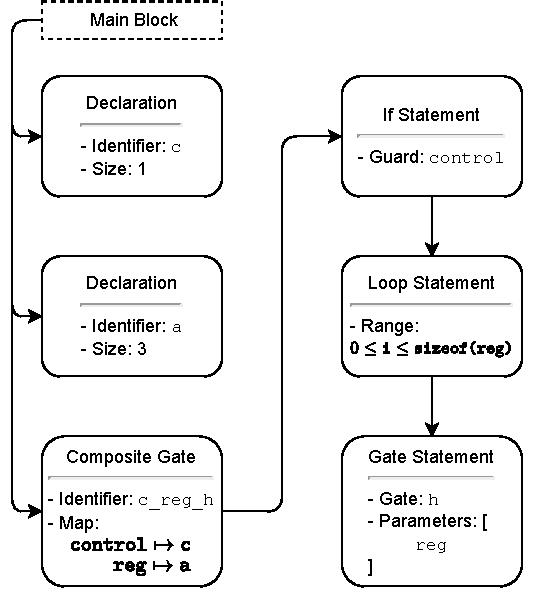
\includegraphics[width=\textwidth]{../figures/drawio/codeGen_sourceCode_example.pdf}
        \caption{The source code representation of the example program.}
        \label{fig:codeGen_sourceCodeRep_example}
    \end{minipage}
    \hfill
    \begin{minipage}{.45\textwidth}
        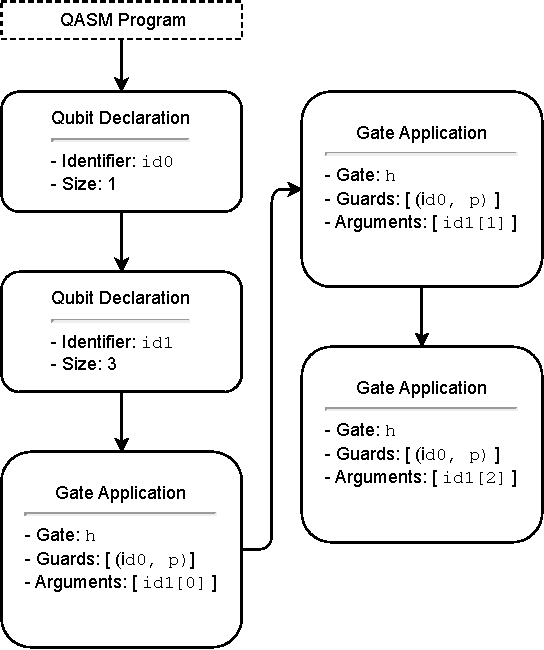
\includegraphics[width=\textwidth]{../figures/drawio/codeGen_targetCode_example.pdf}
        \caption{The target code representation of the example program.}    
        \label{fig:implementation_targetCodeRep_example}
    \end{minipage}
\end{figure}

The first step in the code generation process is the creation of the source code representation. The representation of the code example is depicted in Fig.~\ref{fig:codeGen_sourceCodeRep_example}. 
Here, a dashed box indicates a list, and dashed connections indicate successors in a list, while a solid connection represents one object holding a reference to another.
The root of the source code representation is the main block. While this block is depicted in the diagram, for simplicity, all other code blocks are omitted. The main block contains three different translatables: the declarations and one statement. The two declarations are qubit \texttt{c} and register \texttt{a}, declared in the code example. They are followed by a composite gate statement. This gate contains both a dictionary that maps the gate argument symbols to the given arguments and a reference gate code block, represented by an arrow in the diagram. The body of the composite gate contains an if-statement where \texttt{control} is the control qubit. In turn, the if-statement contains a loop statement that iterates over the range from zero to $\texttt{sizeof(reg)} - 1$. Although the start index is given by a constant value, both the start and end of the range are given as expressions and are evaluated when the loop statement is translated. Lastly, the loop statement contains a gate statement that applies the Hadamard gate to the \texttt{reg[i]} qubit.

Next, the source code representation is translated to the target code representation. The corresponding translation, without the measurement statements added later in the compiler, is depicted in Fig.~\ref{fig:implementation_targetCodeRep_example}. The two declarations are easily translated to their corresponding qubit declarations. However, to ensure the uniqueness of each identifier, they are assigned new identifiers; \texttt{c} becomes \texttt{id0} and \texttt{a} becomes \texttt{id1}. The next three statements, the composite gate, if-, and gate statement, have no target code equivalent. First, the composite gate translation maps the argument symbols used in the gate body to the newly declared qubits. In this case, \texttt{control} is mapped to \texttt{id0} and \texttt{reg} to \texttt{id1}. Then, the body of the gate is translated and inlined. To translate the if-statement, the loop statement needs to be translated first. Here, the loop body is translated for each value in the range of the loop. For this, the start and end expressions are evaluated to zero and two, and, in turn, the loop body is translated three times. For each translation, the new value of the loop iterator \texttt{i} is propagated. The loop body itself only consists of a gate application, where the Hadamard gate is applied to the qubit \texttt{id1[i]} where \texttt{i} changes depending on the iteration. When the loop statement is translated to the three gate applications, the if-statement adds its guard symbol \texttt{id0} to the guard list of each gate application. The result is a sequence of three gate applications, guarded by \texttt{id0} and applying the Hadamard gate to each qubit in the \texttt{id1} register.

Lastly, the remaining step is the conversion from the target code representation to the compiled program code. The final program code, including the language header and measurements, is depicted in Fig.~\ref{fig:codeGen_target_example}. The program object is translated by iterating through all its code objects and calling their translation function \texttt{ToCode}. In the case of the declaration, a qubit is declared if the size is one, while a register is declared for any other size. Since the uniqueness of identifiers is ensured when translating to the target code representation, the identifier of the code object is used for the translation to text. The translation of the gate application adds a control or negative control modifier to the translation, as well as the corresponding control qubits, to the translation depending on the number of positive and negative control qubits. In the example, all gate applications contain only one positive guard. In turn, the resulting statements contain only the control modifier \texttt{ctrl(1) @} with the corresponding qubit as the first argument to the controlled gate. Lastly, a function is called that adds the header and measurement statements to the program.

\begin{figure}
    \centering
    \lstinputlisting[style=QASM]{../figures/code/implementation/codeGen_example.qasm}
    \caption{The OpenQASM translation of the example Luie program.}
    \label{fig:codeGen_target_example}
\end{figure}


\subsection{Expressions}
\label{sec:implementation_expression}
Expressions are used in multiple source code representation objects as a placeholder for a constant value that can only be calculated when the object is translated to the target code. In turn, they need to be created together with the source code object. When such an object is created, the expression subtree of the parse tree is traversed and an expression object is created. The initial function to create the expression differentiates between the different possible cases; for example, in the initial case, either an addition, subtraction, or a term, which can be either a multiplication, division, or a factor, is given. In the case of an addition or subtraction, the two subexpressions are created with a recursive function call, and a combined expression is created. In contrast, when the expression is a term, the corresponding expression creation function is called. Both the expression creation function for the term and factor operate similarly to the function of the expression itself. In turn, the result is an expression object. 

The expression object inherits from an abstract expression class that can be either a binary or unary operation expression, an abstract function expression, an identifier expression, or a constant expression. The expression class takes a generic type parameter with the condition that this type parameter is a number, or more specifically implements the number interface \texttt{INumber}. The type parameter is typically propagated to all subexpressions such that all elements of an expression are of the same type. The type parameter is set when an expression is created and if inferred from the context. For example, in the case of a constant declaration, the given type is used, while for range expressions, the integer type is used.

A binary operation expression is any expression with an operator that operates on two subexpressions. In our case, these are addition, subtraction, multiplication, and division. The expression is evaluated by evaluating the subexpressions and applying the corresponding operation. Similarly, the unary operator expression is an expression with an operator that operates on only one subexpression; the only unary operation is the negation. Again, the expression is evaluated by evaluating the subexpressions and applying the corresponding operation. 

Next, the function expression class is an abstract class from which the different concrete function expression objects are derived. The different possible functions are \texttt{sizeof}, \texttt{power}, \texttt{min}, and \texttt{max}. Firstly, the \texttt{sizeof} expression function takes an identifier and the symbol table as an input and looks up the register information in the table. When evaluated, it returns the size of this register. In contrast, the \texttt{power} function takes two expressions as arguments, evaluates both, and raises the result of the first to the power of the value of the second. Lastly, both the minimum and maximum functions take at least one expression up to arbitrarily many as arguments, evaluate all of them, and return the minimum or maximum value, respectively.

The last two expressions are the identifier and constant expressions. Both differ from all but one expression, the \texttt{sizeof} function expression, in that they are the leaves of the expression tree and do not contain any subexpressions. Similar to the \texttt{sizeof} function expression, the identifier expression contains the symbol of either a constant or loop iterator; when it is created, it retrieves the respective information for the symbol table, and, when it is evaluated, the result is the value of the symbol. In the case of the loop iterator, the current value is used. If the type of the identifier does not correspond to the type of the expression, the value is cast. 
In contrast, the constant expression simply contains a value of the type given as the type parameter; when evaluated, it returns the value.